\section{Related work} \label{related_work}

In order to have a better understanding of YOLO, we aim in section to describe other well known methods.

\subsection{Single Shot MultiBox Detector}

Single shot MultiBox Detector (SSD) \cite{ssd} is another example of an object detection system that achieves real-time performance, encapsulating all operations in a single deep neural network. Like YOLO, this helps SSD to outperform in terms of speed previous approaches that use multiple stages in detection such as R-CNN. 
     
The network architecture is similar to the one of YOLO, or to the single shot object detectors architectures in general. As such, the network is composed mainly of two parts, and optionally the neck. The first one is the same and consists of what is called the base network, which is a truncated version of an image classifier, where the classification layers are removed, that is used to extract features. On top of the base network, several structures specific to object detection are added.
        
The key features of SSD are the multi-scale feature maps, convolutional predictors, and default boxes. 
        
        \begin{figure}[h]
          \centering
          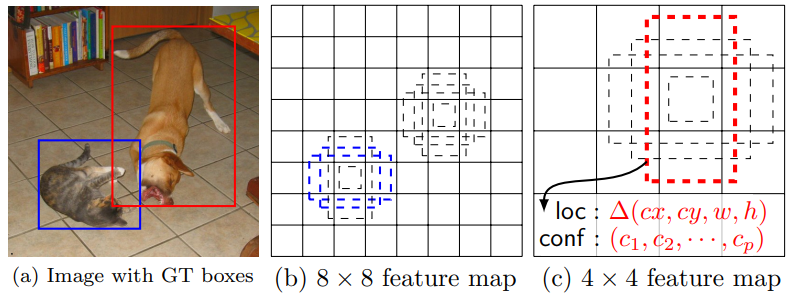
\includegraphics[scale=0.6]{images/ssd.png}
          \caption{Visualization of the feature maps used in SSD \cite{ssd}}
          \label{ssdImg}
        \end{figure}
        
The main difference between this method and YOLO is that to the base network, there are appended several convolutional layers that decrease progressively in size the feature map from the base network. This way predictions are made for each newly added layer, therefore, the predictions are made at various scales, as it is depicted in Fig. \ref{ssdImg}. 
        
Each cell in each feature map has associated K default bounding boxes, whose positions are relative to their cell. Then for each box several kernels of size $3 \times 3 \times P$, where $M \times N$ is the size of the feature map and P is the number of channels, are used to predict C class probabilities and 4 offsets to the respective box. This means that each box uses $(C+4)\cdot K$ filters, therefore the size of the predictions is $(C+4)  \times  K \times M \times N$.
        
During training, the outputs need to be assigned to their corresponding ground truths. Then the loss function and backpropagation are applied end-to-end. Furthermore, the set of default boxes and scales is chosen, and hard negative mining and data augmentation strategies are used.
        
For matching the outputs, each ground truth box is associated with the default box with the highest Jaccard overlap. The novel approach here is that the default boxes are also matched with any ground truth box with a Jaccard overlap higher than a threshold. This allows predictions with high scores for multiple overlapping default boxes.
        
%The loss is a weighted sum between confidence loss and localization loss.
        
Another crucial part is choosing scales and aspect ratios for the default boxes. Each feature map has a specific scale, distributed evenly between two values. The aspect ratios are chosen from a predefined set. The width and height are computed using the scale and the aspect ratio. The center is chosen based on the feature map cell size.
        
The matching steps produce more negatives than positives. This introduces an imbalance, and to fix this, the negatives are filtered by their confidence loss so that a ratio of three to one is kept between the negatives and positives.
        
%Also, data augmentation is used. During training for each image either a patch is randomly sampled, a path is sampled so that the minimum Jaccard overlap with the objects is higher than a threshold, or the original image is used. After this, the image is resized and flipped with a probability of 0.5, and some photometric distortions are applied.

\subsection{Region based convolutional neural networks}

This type of method falls into the category of two-stage object detectors. Traditionally, there was a clean separation in terms of performance between this type of object detectors and the one stage class of object detectors, but with time, both types of methods became better in what they lacked by bringing several optimizations over the original architecture. Two stage methods gained speed and one stage methods gained accuracy for example.

In Fig. \ref{rcnnImg} we can observe why this method is a two-stage type of method. Basically, the first stage is to extract from the input image a lot of region proposals or region of interests. Ideally, these region proposals contain objects of interest and will represent the final bounding box. Here we can observe the fundamental difference between two-stage methods and YOLO, or one-stage methods in general. In one-stage methods, the bounding boxes are obtained through regression, while in two-stage methods, they are extracted beforehand. It is important to note that R-CNN is agnostic to the way region proposals are extracted from the input image, as the authors mention. One way the region proposals can be extracted is by selective search, which is the method adopted originally by the authors and it does not involve any learning. Another way is to obtain them through a what is called a region proposal network that is a fully convolutional network capable of predicting both bounding boxes and objectness scores.

\begin{figure}[h]
  \centering
  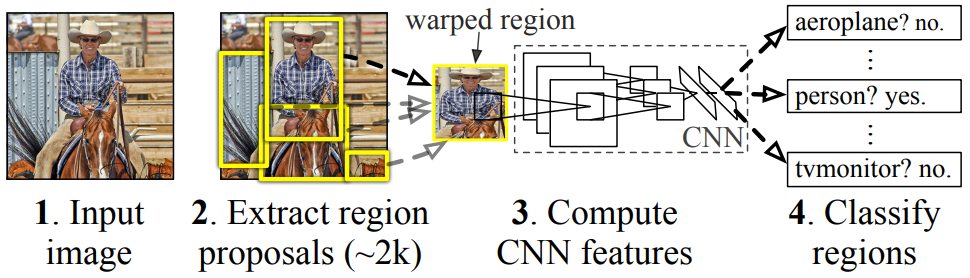
\includegraphics[scale=0.4]{images/rcnn.png}
  \caption{Two stage pipeline used in R-CNN \cite{rcnn}}
  \label{rcnnImg}
\end{figure}

Region proposal is a complex domain and it deserves focused research on it's own. The idea is that it is crucial for two-stage method to have good proposals in order to achieve high performance. This could be seen as a downside compared to it's counterparts, the one-stage methods, because it adds a layer of extra complexity. Also, the density of region proposals is crucial, this also being related to a more general problem in object detection, that of defining positives. Thus, if there aren't enough proposals, the network performance will be limited in the sense that it will not be able to find all objects and the recall can be affected.

The second step is to take the region proposals and classify them. Optionally, the region proposals can be further refined before being classified. The classification can be done in several ways such as with artificial neural networks, convolutional neural networks or support vector machines.

The final predictions are composed from the bounding boxes given by the region proposals and the classification scores resulted from the second stage.

This method as it is can achieve good performance in terms of precision but it lacks speed. This is mostly due to the fact that many region proposals are actually overlapping, thus there are a lot of extra computations that have a negative impact on the speed. This was further optimized in Fast R-CNN \cite{fastRcnn} by introducing a convolutional neural network as a preliminary step before selective search in order to then compute region proposals on the processed feature maps using region of interest pooling. In this way, the feature extraction becomes a shared computation. Another optimization is proposed in Faster R-CNN \cite{fasterRcnn} and it consists of replacing selective search with a region proposal network, that can learn to predict a set of object proposals, together with their objectness scores directly from the extracted feature maps, resulted by passing the input image through a convolutional neural network. These optimizations greatly reduce the inference time, and maintain good performance, but the method still lacks behind one-stage methods such as YOLO in terms of speed.


